% A (minimal) template for problem sets and solutions using the exam document class

% Organization:
%% Define new commands, macros, etc. in macros.tex
%% Anything that you would put before \begin{document} should go in prelude.tex

%% For multiple psets, each should get its own file to \input into main with a \section{}

\documentclass[answers]{exam}
\usepackage{amsmath}
\usepackage{amsthm}
\usepackage{amsfonts}
\usepackage{amssymb}
\usepackage{mathrsfs}
\usepackage{mathtools}
\usepackage{hyperref}
\usepackage{cancel}
\usepackage{xcolor}
\usepackage{graphicx}
\usepackage{subfig}
\usepackage{caption}
\usepackage{braket}
\usepackage{bm}
\usepackage[utf8]{inputenc}
\usepackage[english]{babel}
\usepackage[noabbrev]{cleveref}
\renewcommand{\qedsymbol}{$\blacksquare$}
\renewcommand{\questionlabel}{\alph{question}.}
\newcommand{\highlight}[1]{%
  \colorbox{red!50}{$\displaystyle#1$}}
\newcommand{\hlgreen}[1]{%
  \colorbox{green!50}{$\displaystyle#1$}}
\newcommand{\hlyellow}[1]{%
  \colorbox{yellow!90}{$\displaystyle#1$}}
\newcommand{\hlblue}[1]{%
  \colorbox{blue!20}{$\displaystyle#1$}}

\pagestyle{headandfoot}
\runningheadrule
\firstpageheader{Uriel A. Aceves R.}{Computational Many-Body Theory}{Homework 6}
\runningheader{Uriel A. Aceves R.}
{Computational Many-Body Theory}
{Homework 6}
\firstpagefooter{Due 28.06.}{Page \thepage\ of \numpages}{SS18}
\runningfooter{Due 28.06.}{Page \thepage\ of \numpages}{SS18}

\begin{document}

%% \union - Example: \union{j \in J}{A_j}
\newcommand{\union}[2]{\underset{#1}\bigcup #2}

%% \inter - like \union, but with \bigcap
\newcommand{\inter}[2]{\underset{#1}\bigcap #2}

%% Content goes here

\section{Integral with Fermi-sphere constraints}
%\begin{questions}
\question{
Show that those operators are fermionic
}
\begin{solution}
  By definition, fermion operators must satisfy the following anti-commutation rules
  \begin{itemize}
    \item $\{a_{\alpha,\sigma},a_{\alpha',\sigma'}\} = 0.$
    \item $\{a^\dagger_{\alpha,\sigma},a^\dagger_{\alpha',\sigma'}\} = 0.$
    \item $\{a_{\alpha,\sigma},a^\dagger_{\alpha',\sigma'}\} = \delta_{\alpha, \alpha'}\delta_{\sigma,\sigma'}.$
  \end{itemize}
  Now we are going to prove that if $\hat{c}_{m,\zeta}$ is a fermion operator then the linear combinations
  \begin{eqnarray}
    \hat{d}_\mu = \sum_m \alpha_m\hat{c}_{m,\mu},\\
    \hat{d}^\dagger_\mu = \sum_m \alpha^*_m\hat{c}^\dagger_{m,\mu},
  \end{eqnarray}
  are fermion operators too.

  So we are going to prove they obey the previously mentioned anti-commutation rules. We will use the linearity property of the anti-commutator shown in eq. \ref{linear}

  \begin{equation}
    \{\alpha A + \beta B, \gamma C + \delta D\} =   \{\alpha A, \gamma C\} +  \{\alpha A ,\delta D\} +   \{ \beta B, \gamma C \} +   \{ \beta B, \delta D\}.
    \label{linear}
  \end{equation}
  Let's go then,
  \begin{equation}
    \begin{aligned}[b]
      \{\hat{d}_\mu, \hat{d}_\nu\} &= \left\{\sum_m \alpha_m\hat{c}_{m,\mu}, \sum_n \alpha_n\hat{c}_{n,\nu}\right\},\\
      &= \sum_{m,n} \alpha_m \alpha_n \cancelto{0}{\{\hat{c}_{m,\mu},\hat{c}_{n,\nu}\}},\\
      &= 0.
    \end{aligned}
  \end{equation}
  \begin{equation}
    \begin{aligned}[b]
      \{\hat{d}^\dagger_\mu, \hat{d}^\dagger_\nu\} &= \left\{\sum_m \alpha_m^*\hat{c}^\dagger_{m,\mu}, \sum_n \alpha_n^*\hat{c}^\dagger_{n,\nu}\right\},\\
      &= \sum_{m,n} \alpha_m^* \alpha_n^* \cancelto{0}{\{\hat{c}^\dagger_{m,\mu},\hat{c}^\dagger_{n,\nu}\}},\\
      &= 0.
    \end{aligned}
  \end{equation}
  \begin{equation}
    \begin{aligned}[b]
      \{\hat{d}_\mu, \hat{d}^\dagger_\nu\} &= \left\{\sum_m \alpha_m\hat{c}_{m,\mu}, \sum_n \alpha_n^*\hat{c}^\dagger_{n,\nu}\right\},\\
      &= \sum_{m,n} \alpha_m \alpha_n^* \cancelto{\delta_{m,n}\delta_{\mu,\nu}}{\{\hat{c}_{m,\mu},\hat{c}^\dagger_{n,\nu}\}},\\
      &= \sum_{m,n} \alpha_m \alpha_n^*\delta_{m,n}\delta_{\mu,\nu},\\
      &= \cancelto{1}{\sum_{m} \alpha_m \alpha_m^*}\delta_{\mu,\nu},\\
      &= \delta_{\mu,\nu}.
    \end{aligned}
  \end{equation}
  Where we used the fact that $\hat{c}$ are fermion operators, and in the last one we used additionally $\sum_m \alpha_m^2 = 1$. Since the $\hat{d}$ operators comply with the anti-commutation rules for fermion operators we conclude that they are indeed fermion operators. $\blacksquare$
\end{solution}

\question{Majorana operators}
\begin{solution}
  Now we are going to prove basically the same but for the next operators (I changed the labels to make the life easier for me)
  \begin{eqnarray}
    \hat{\gamma}_+ = \frac{1}{\sqrt{2}}\left(\hat{d} + \hat{d}^\dagger \right)\\
    \hat{\gamma}_- = \frac{i}{\sqrt{2}}\left(\hat{d} - \hat{d}^\dagger \right)
  \end{eqnarray}

  \begin{equation}
    \begin{aligned}[b]
      \{\hat{\gamma}_\pm,\hat{\gamma}_\pm \} &= \left\{\frac{\alpha_\pm}{\sqrt{2}}\left(\hat{d} \pm \hat{d}^\dagger \right),\frac{\alpha_\pm}{\sqrt{2}}\left(\hat{d} \pm \hat{d}^\dagger \right)\right\},\\
      &= \frac{\cancelto{\pm 1}{\alpha^2_\pm}}{2}\left\{\hat{d} \pm \hat{d}^\dagger ,\hat{d} \pm \hat{d}^\dagger \right\},\\
      &= \frac{\pm 1}{2}\left(\cancelto{0}{\left\{\hat{d} ,\hat{d} \right\}}  \pm \cancelto{1}{\left\{\hat{d}, \hat{d}^\dagger \right\}} \pm \cancelto{1}{\left\{  \hat{d}^\dagger ,\hat{d}\right\}} + \cancelto{0}{\left\{\hat{d}^\dagger ,\hat{d}^\dagger \right\}}\right),\\
      &= 1.
    \end{aligned}
  \end{equation}
  Where $\alpha_+ = 1$, and $\alpha_- = i$.
  \begin{equation}
    \begin{aligned}[b]
      \{\hat{\gamma}_\pm,\hat{\gamma}_\mp \} &= \left\{\frac{\alpha_\pm}{\sqrt{2}}\left(\hat{d} \pm \hat{d}^\dagger \right),\frac{\alpha_\mp}{\sqrt{2}}\left(\hat{d} \mp \hat{d}^\dagger \right)\right\},\\
      &= \frac{\cancelto{i}{\alpha^2_\pm}}{2}\left\{\hat{d} \pm \hat{d}^\dagger ,\hat{d} \mp \hat{d}^\dagger \right\},\\
      &= \frac{i}{2}\left(\cancelto{0}{\left\{\hat{d} ,\hat{d} \right\}}  \pm \cancelto{1}{\left\{\hat{d}, \hat{d}^\dagger \right\}} \mp \cancelto{1}{\left\{  \hat{d}^\dagger ,\hat{d}\right\}} + \cancelto{0}{\left\{\hat{d}^\dagger ,\hat{d}^\dagger \right\}}\right),\\
      &= 0.
    \end{aligned}
  \end{equation}
  As a conclusion we see that
  \begin{equation}
    \{\hat{\gamma}_\mu , \hat{\gamma}_\nu\} = \delta_{\mu \nu}.
    \label{commu}
  \end{equation}

  Finally we need to express the number operator in terms of $\hat{\gamma}_+$ and $\hat{\gamma}_-$. The trick we are going to use here is an old known if we have solved the harmonic oscillator with creation and annihilation operators. We can easily show that
  \begin{eqnarray}
    \hat{d}^\dagger = \frac{\hat{\gamma}_+ + i\hat{\gamma}_-}{\sqrt{2}},\\
    \hat{d} = \frac{\hat{\gamma}_+ - i\hat{\gamma}_-}{\sqrt{2}},
  \end{eqnarray}
  therefore
  \begin{equation}
    \begin{aligned}[b]
      \hat{n} &= \hat{d}^\dagger \hat{d},\\
      &= \left(\frac{\hat{\gamma}_+ + i\hat{\gamma}_-}{\sqrt{2}}\right)\left(\frac{\hat{\gamma}_+ - i\hat{\gamma}_-}{\sqrt{2}}\right),\\
      &= \frac{(\hat{\gamma}_+ + i\hat{\gamma}_-)(\hat{\gamma}_+ - i\hat{\gamma}_-)}{2},\\
      &= \frac{\hat{\gamma}_+\hat{\gamma}_+ - i\hat{\gamma}_+\hat{\gamma}_- + i\hat{\gamma}_- \hat{\gamma}_+ + \hat{\gamma}_-\hat{\gamma}_-}{2}
      \label{n:almost}
    \end{aligned}
  \end{equation}
  If we use what we know from eq. \ref{commu} we will notice that
  \begin{equation}
    \begin{aligned}[b]
      \{\hat{\gamma}_\pm,\hat{\gamma}_\mp \} = \hat{\gamma}_\pm\hat{\gamma}_\mp+ \hat{\gamma}_\mp\hat{\gamma}_\pm = 0,\\
      \Rightarrow \hat{\gamma}_\pm\hat{\gamma}_\mp = - \hat{\gamma}_\mp\hat{\gamma}_\pm,
      \label{help1}
    \end{aligned}
  \end{equation}
  and also
  \begin{equation}
    \begin{aligned}[b]
      \{\hat{\gamma}_\pm,\hat{\gamma}_\pm \} = \hat{\gamma}_\pm\hat{\gamma}_\pm+ \hat{\gamma}_\pm\hat{\gamma}_\pm = 2 \hat{\gamma}_\pm\hat{\gamma}_\pm = 1,\\
      \Rightarrow \hat{\gamma}_\pm\hat{\gamma}_\pm = \frac{1}{2}.
      \label{help2}
    \end{aligned}
  \end{equation}
  Using eqs. \ref{help1}-\ref{help2} in eq. \ref{n:almost} we will have
  \begin{equation}
    \begin{aligned}[b]
      \hat{n} &= \frac{\hat{\gamma}_+\hat{\gamma}_+ - i\hat{\gamma}_+\hat{\gamma}_- + i\hat{\gamma}_- \hat{\gamma}_+ + \hat{\gamma}_-\hat{\gamma}_-}{2}\\
      &=\frac{1/2 + 2i\hat{\gamma}_- \hat{\gamma}_+ + 1/2}{2}\\
      &=\frac{1}{2} + i\hat{\gamma}_- \hat{\gamma}_+.
      \label{n:almost}
    \end{aligned}
  \end{equation}
\end{solution}
\end{questions}


% \includegraphics[width=75mm]{}
%
%
%  \captionof{figure}{}\label{}\vspace{0.5cm}


\section{Density of states}
%\begin{questions}
\question{
Spin
}
\begin{solution}
 The first step we need to take is expanding the field operators on the given basis
 \begin{eqnarray}
   \Phi_{\sigma}(\vec{r}) = \sum_{k} \psi_{k}(\vec{r})c_{k,\sigma},\label{field:1}\\
   \Phi_{\sigma}(\vec{r}) = \sum_{n,l,m} \psi_{n,l,m}(\vec{r})c_{n,l,m,\sigma}\label{field:2}
 \end{eqnarray}
 And their respective dagger operators. From Fetter and Walecka we know how to obtain the second-quantized operator from the first-quantization operator.
 \begin{equation}
   \hat{s_i} = \sum_{\sigma,\sigma'} \Phi_\sigma^\dagger(\vec{r})s_i\Phi_{\sigma'}(\vec{r}),\label{dens}
 \end{equation}
 inserting eq. \ref{field:1} into eq. \ref{dens}, and pulling up the spin index explicitly, yields
 \begin{equation*}
   \begin{aligned}[b]
     \hat{s_i} &= \sum_{k,k',\sigma, \sigma'} \bra{\psi_{k}}\bra{\sigma} s_i  \ket{\sigma'}\ket{\psi_{k'}}c^\dagger_{k,\sigma}c_{k',\sigma'},\\
     &= \sum_{k,k',\sigma, \sigma'} \braket{\psi_{k}|\psi_{k'}}\bra{\sigma} s_i  \ket{\sigma'}c^\dagger_{k,\sigma}c_{k',\sigma'}
   \end{aligned}
 \end{equation*}
 \begin{equation}
   \begin{aligned}[b]
     &= \sum_{k,k',\sigma, \sigma'} \delta_k^{k'}\bra{\sigma} s_i  \ket{\sigma'}c^\dagger_{k,\sigma}c_{k',\sigma'}\\
     &= \hlgreen{\sum_{k,\sigma, \sigma'}\bra{\sigma} s_i  \ket{\sigma'}c^\dagger_{k,\sigma}c_{k',\sigma'}}.
   \end{aligned}
 \end{equation}
 We can use the same trick, but now plugging eq. \ref{field:2} into eq. \ref{dens}
 \begin{equation}
   \begin{aligned}[b]
     \hat{s_i} &= \sum \bra{\psi_{n,l,m}}\bra{\sigma} s_i  \ket{\sigma'}\ket{\psi_{n',l',m'}}c^\dagger_{n,l,m,\sigma}c_{n',l',m',\sigma'},\\
     &= \sum \braket{\psi_{n,l,m}|\psi_{n',l',m'}}\bra{\sigma} s_i  \ket{\sigma'}c^\dagger_{n,l,m,\sigma}c_{n',l',m',\sigma'},\\
     &= \sum \delta_{nlm}^{n'l'm'}\bra{\sigma} s_i  \ket{\sigma'}c^\dagger_{n,l,m,\sigma}c_{n',l',m',\sigma'},\\
     &= \hlgreen{\sum_{nlm\sigma\sigma'} \bra{\sigma} s_i  \ket{\sigma'}c^\dagger_{n,l,m,\sigma}c_{n,l,m,\sigma'}.}
   \end{aligned}
 \end{equation}
 Where the first three sums were performed over $n,l,m,\sigma,n',l',m',\sigma'$. The highlighted equations are indeed the total spin operators for the two chosen basis.
\end{solution}
\end{questions}


\section{Reciprocal lattice}
\begin{questions}
\question{
Sinc(x) definition of the delta function
}
\begin{solution}

First we will calculate the given integral

\begin{equation}
  \begin{aligned}[b]
    \frac{1}{2\pi} \int_{-Z}^Z e^{ikx}dk &= \left.\frac{e^{ikx}}{2\pi ix} \right|_{-Z}^Z ,\\
    &= \frac{e^{iZx} - e^{-iZx}}{2\pi ix},\\
    &= \frac{1}{\pi x}\frac{e^{iZx} - e^{-iZx}}{2i},\\
    &= \frac{\sin(Zx)}{\pi x}.
    \label{int:delt}
  \end{aligned}
\end{equation}

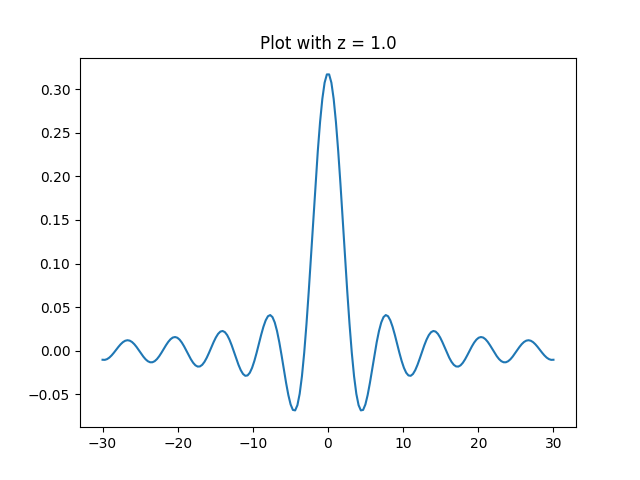
\includegraphics[width=50mm]{delt1.png}
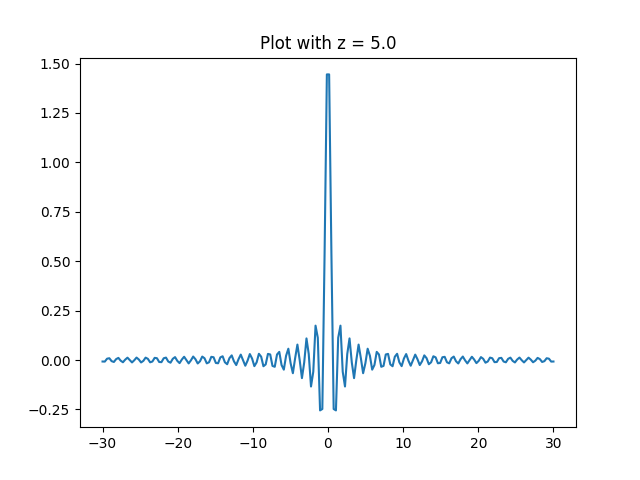
\includegraphics[width=50mm]{delt5.png}
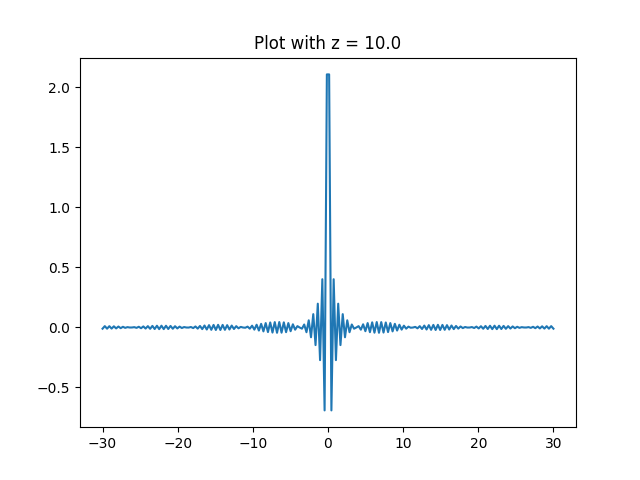
\includegraphics[width=50mm]{delt10.png}\label{del:plots}

\hspace{25mm}a)\hspace{47mm}b)\hspace{48mm}c)

 \captionof{figure}{Plots for eq. \ref{int:delt} using a) $Z=1$, b) $Z=5$, and c) $Z=10$}
 \vspace{1cm}

 \textbf{Where does it have its maximum value?} At x=0.\\

 \textbf{What happens when increasing Z?} The peak rises but also narrows.\\

 \end{solution}

 \question{The integral of $\delta$ is one.}
 \begin{solution}

 Now we need to show that the integral of delta is one

 \begin{equation}
   \begin{aligned}[b]
     \int_{-\infty}^\infty \delta(x) dx &= \int_{-\infty}^\infty \frac{1}{2\pi} \lim_{Z\rightarrow \infty} \int_{-Z}^Z e^{ikx}dk,\\
     &= \int_{-\infty}^\infty \lim_{Z\rightarrow \infty} \frac{\sin(Zx)}{\pi x},\quad  \textnormal{using eq. \ref{int:delt}},\\
     &=\lim_{Z\rightarrow \infty} \int_{-\infty}^\infty  \frac{\sin(Zx)}{\pi x}, \quad \textnormal{linearity},\\
     &= \frac{1}{\pi}\lim_{Z\rightarrow \infty} \int_{-\infty}^\infty \frac{\sin(x')}{ x'}dx', \quad \textnormal{change of variable $x'=Zx$},\\
     &= \frac{1}{\pi}\lim_{Z\rightarrow \infty} \pi,\\
     &= \frac{\pi}{\pi} = 1 \quad _\blacksquare. \label{integral}
   \end{aligned}
 \end{equation}
 Being strict we should have changed the $Z$ on the limit when we changed variable, but as we saw the final result of the integral was not affected by the value of $Z$. So we can omit that step in order to avoid unnecessary calculations.
\end{solution}

\question{Fourier transform of $\delta$}
\begin{solution}
  Let's begin with the definition
  \begin{equation*}
    \begin{aligned}
      \delta(k') &= \int_{-\infty}^\infty e^{-ik'x}\delta(x)dx,\\
      &= \int_{-\infty}^\infty e^{-ik'x}\left(\frac{1}{2\pi}\int_{-\infty}^\infty e^{ikx}dk\right)dx, \quad \textnormal{definition of $\delta(x)$,}\\
      &= \frac{1}{2\pi}\int_{-\infty}^\infty \int_{-\infty}^\infty e^{-ik'x} e^{ikx}dkdx,\\
      &= \frac{1}{2\pi}\int_{-\infty}^\infty \int_{-\infty}^\infty  e^{i(k-k')x}dkdx,\\
      &= \frac{1}{2\pi}\int_{-\infty}^\infty \int_{-\infty}^\infty  e^{ik''x}dk''dx, \quad \textnormal{variable change $k'' = k-k'$},\\
      &= \int_{-\infty}^\infty \left( \frac{1}{2\pi}\int_{-\infty}^\infty  e^{ik''x}dk''\right)dx,\\
      &= \int_{-\infty}^\infty \delta(x) dx, \quad \textnormal{by definition},\\
      &= 1, \quad \textnormal{using eq. \ref{integral}}.
    \end{aligned}
  \end{equation*}

\end{solution}

\question{Properties of Dirac's delta}
\begin{solution}
 Here we show a couple of properties of this distribution
 \begin{eqnarray}
   \int_{-\infty}^\infty f(x)\delta(x)dx = f(0).\\
   \int_{-\infty}^\infty \delta(\alpha x)dx = \frac{1}{|\alpha|}.\\
   \delta(-x) = \delta(x).\\
   \int_{-\infty}^\infty f(t)\delta(t-T)dx = f(T).\\
   \int_{-\infty}^\infty f(x)\delta(x-a) = \int_{-\infty}^\infty f(a)\delta(x-a).\\
   \int_{-\infty}^\infty \delta(a-x)\delta(x-b)dx = \delta(a-b).
 \end{eqnarray}
\end{solution}

\question{Properties of Fourier transforms}
\begin{solution}
We will denote the Fourier transform operation  with a hat. For $a,b\in \mathbb{C}$, if $h(x) = af(x) + bg(x)$ then
\begin{eqnarray}
  \hat{h}(\xi) = a\hat{f}(\xi) +b\hat{g}(\xi).
\end{eqnarray}
For $x_0\in \mathbb{R}$, if $h(x)=f(x-x_0)$, then
\begin{equation}
  \hat{h}(\xi) = e^{-2\pi ix_0\xi}\hat{f}(\xi).
\end{equation}
For $\xi_0\in \mathbb{R}$, if $h(x)=e^{2\pi ix\xi_0}f(x)$, then
\begin{equation}
  \hat{h}(\xi) = \hat{f}(\xi - \xi_0).
\end{equation}
For $a\neq 0 \in \mathbb{R}$ if $h(x) = f(ax)$ then
\begin{equation}
  \hat{h}(\xi) = \frac{1}{|a|}f\left(\frac{\xi}{a}\right).
\end{equation}
If $h(x) = \overline{f(x)}$, then
\begin{equation}
  \hat{h}(\xi) = \overline{\hat{f}(-\xi)}.
\end{equation}
But we have to be careful with those $2\pi$ factors because they depend on the definition of the Fourier transform, and the inverse Fourier transform.
\end{solution}

\end{questions}

% \includegraphics[width=75mm]{}\label{}
%
%
%  \captionof{figure}{}


\end{document}
